\ifdefined\COMPLETE
\else
\documentclass[11pt]{article}
\usepackage[french, english]{babel}
\usepackage[utf8]{inputenc}
\usepackage{graphicx}
\usepackage{framed}
\usepackage[normalem]{ulem}
\usepackage{amsmath}
\usepackage{amsthm}
\usepackage{amssymb}
\usepackage{amsfonts}
\usepackage{enumerate}
\usepackage{import}
\usepackage[top=1 in,bottom=1in, left=1 in, right=1 in]{geometry}
\usepackage{listingsutf8}
\usepackage{color}
\usepackage{float}
\usepackage{graphicx}
\usepackage{subcaption}
\usepackage[toc,page]{appendix}
\usepackage{multicol}
\usepackage{wrapfig}
\usepackage{sidecap}

\floatstyle{boxed} 
\restylefloat{figure}
\definecolor{mygreen}{rgb}{0,0.6,0}
\definecolor{mygray}{rgb}{0.5,0.5,0.5}
\definecolor{mymauve}{rgb}{0.58,0,0.82}
\newcommand{\dt}{\partial_t}
\newcommand{\Tl}{\frac{T}{\lambda}}
\theoremstyle{definition}
\newtheorem{definition}{Définition}[section]
\DeclareMathOperator*{\argmax}{arg\,max}
\DeclareMathOperator*{\argmin}{arg\,min}
 


\lstset{ 
  backgroundcolor=\color{white},   % choose the background color; you must add \usepackage{color} or \usepackage{xcolor}; should come as last argument
  basicstyle=\footnotesize,        % the size of the fonts that are used for the code
  breakatwhitespace=false,         % sets if automatic breaks should only happen at whitespace
  breaklines=true,                 % sets automatic line breaking
  captionpos=b,                    % sets the caption-position to bottom
  commentstyle=\color{mygreen},    % comment style
  deletekeywords={...},            % if you want to delete keywords from the given language
  escapeinside={\%*}{*)},          % if you want to add LaTeX within your code
  extendedchars=true,              % lets you use non-ASCII characters; for 8-bits encodings only, does not work with UTF-8
  firstnumber=1000,                % start line enumeration with line 1000
  frame=single,	                   % adds a frame around the code
  keepspaces=true,                 % keeps spaces in text, useful for keeping indentation of code (possibly needs columns=flexible)
  keywordstyle=\color{blue},       % keyword style
  language=Python,                 % the language of the code
  morekeywords={*,...},            % if you want to add more keywords to the set
  numbers=left,                    % where to put the line-numbers; possible values are (none, left, right)
  numbersep=5pt,                   % how far the line-numbers are from the code
  numberstyle=\tiny\color{mygray}, % the style that is used for the line-numbers
  rulecolor=\color{black},         % if not set, the frame-color may be changed on line-breaks within not-black text (e.g. comments (green here))
  showspaces=false,                % show spaces everywhere adding particular underscores; it overrides 'showstringspaces'
  showstringspaces=false,          % underline spaces within strings only
  showtabs=false,                  % show tabs within strings adding particular underscores
  stepnumber=2,                    % the step between two line-numbers. If it's 1, each line will be numbered
  stringstyle=\color{mymauve},     % string literal style
  tabsize=2,	                   % sets default tabsize to 2 spaces
  title=\lstname                   % show the filename of files included with \lstinputlisting; also try caption instead of title
}
\lstset{inputencoding=utf8/latin1}
\newcommand{\Dt}{\Delta t}
\newcommand{\Dx}{\Delta x}
 %file containing all the used libraries
\begin{document}
\fi
\section{Recherche de la vitesse d'onde des solutions progressives de l'Équation fluide complète du champignon.}
Le but de cette section est de montrer comment l'on peut obtenir la vitesse d’onde pour l’équation du champignon complète:  
\begin{equation}  \left\{
                \begin{array}{ll}
                \dt\mu + \nabla(\mu v) = f(C)(\mu + \rho) -\mu\rho \\
                   \dt(\mu v)+\nabla(\mu v\times v) +T\nabla\mu=-\lambda\mu v+\mu\nabla C-\mu v \rho \\
                 \dt\rho=  F(v) \mu \\
                  \dt C = -b\rho C.
                \end{array}
              \right.
\end{equation} 
En effet dans les sections précédentes nous avons travaillés dans le cas $\lambda$ et $T$ très grands ce qui simplifiait les équations.\\
Cependant nous avons pu voir que, comme pour l’équation de Fisher KPP, pour une donnée initiale à support compact, la solution tend vers une solution d'onde et que la vitesse d'onde est déterminée par la plus petite vitesse (en valeur absolue) donnée par la condition d'amortissement fort autour de l'état initial.\\
Nous allons alors adopter la même stratégie pour l’équation complète.\\
Ici nous allons linéariser autour de l’état $(\mu,\rho,C,v) = (0,0,C_0,v)$.\\
Equation d'onde pour le fluide:\\
Soit $s$ la vitesse d'onde, $y=x-st$, par le même argument de symétrie que pour l’équation de  ``KPP avec mémoire", nous allons se placer dans le cas $s<0$. Avec abus de notation $ :(x,t) = :(y)$, où $y=x-st$, l’équation d'onde pour le fluide est:
\begin{equation}\label{eq:FWS_BDNG}  \left\{
                \begin{array}{ll}
                -s\mu' + (\mu v)' = f(C)(\mu + \rho) -\mu\rho \\
                   -s (\mu v)'+(\mu v\times v)' +T\mu'=-\lambda\mu v+\mu C'-\mu v \rho \\
                 -s \rho '=  F(v) \mu \\
                  -sC' = -b\rho C.
                \end{array}
              \right.
\end{equation} 
Linéarisation autour de l’état  $(\mu,\rho,C,v) = (0,0,C_0,v)$: \\
On pose $f(C_0) = f_0$, et on cherche des solutions de la forme $\rho = \rho_0 \exp(Xy)$ autour de $\rho=0$.\\ 
On obtient en intégrant la quatrième ligne $C= C_0 - \frac{b\rho_0 C_0}{X}\exp(Xy).$\\
La troisième ligne donne: $-sX\rho_0\exp(Xy)=F_0\mu$ donc $\mu = \frac{-sX\rho_0}{F_0}\exp(Xy)$.\\
Autour de $(\mu,\rho,C,v) = (0,0,C_0,v)$, la première ligne donne: $-s\mu' + (\mu v)' = f_0(\mu + \rho)$ car on peut négliger $\mu\rho$ devant $\mu$ et $\rho$ . On a donc \begin{equation}
	(\mu v)'=(f_0\rho_0-\frac{sXf_0\rho_0}{F_0}-\frac{s^2X^2\rho_0}{F_0})\exp(Xy)
\end{equation}
donc \begin{equation}
	\mu v = (\frac{f_0\rho_0}{X}- \frac{f_0s\rho_0}{F_0}-\frac{s^2X\rho_0}{F_0})\exp(Xy).
\end{equation}
Ainsi \begin{equation}
	v= \frac{\mu v}{\mu} = v_0 = s + \frac{f_0}{X}-\frac{f_0F_0}{X^2s}  .
\end{equation}
La deuxième ligne donne $-s (\mu v)'+(\mu v\times v)' +T\mu'=-\lambda\mu v+\mu C'-\mu v \rho$. \\
On peut ici négliger $\mu v\rho$ et $\mu C'$ devant $\mu v$. On a donc: \begin{equation}
	(-v_0sX\mu_0 + v_0^2X\mu_0 +T\mu_0X)\exp(Xy) = -\lambda\mu_0v_0\exp(Xy)
\end{equation}
donc \begin{equation}
	-sXv_0 + v_0^2X+ TX = -\lambda v_0.
\end{equation}
En multipliant par $X^2$ et en substituant $v_0 =  s + \frac{f_0}{X}-\frac{f_0F_0}{X^2s}$ on a alors l’équation caractéristique:
\begin{equation} \label{eq:P}
	X^4(Ts^2) + X^3(\lambda + f_0)s^3+ X^2(f_0^2s^2+ \lambda f_0 s^2 - f_0F_0s^2)+ X(-sF_0f_0)(\lambda+2f_0) + f_0^2F_0^2=0.
\end{equation}
En posant $Y = sX$ on obtient: \begin{equation}
	A(Y) \equiv Y^4+\frac{s^2}{T}P_3(Y)=0 \label{eq:PY}
\end{equation} où \begin{equation}
		P_3(Y) \equiv  Y^3(\lambda + f_0)+ Y^2(f_0^2+ \lambda f_0 - f_0F_0)- Y(F_0f_0(\lambda+2f_0)) + f_0^2F_0^2
\end{equation} est un polynôme de degré 3 dont les coefficients ne dépendent que des données $f_0$, $F_0$, $\lambda$ et $T$. \\
\subsection{Condition d'amortissement fort}
La vitesse recherchée est le plus petit $s>0$ (ou plus grand $s<0$ ) tel que le polynôme de degré 4 $A$ défini dans \ref{eq:PY} possede quatre racines réelles (comptées avec multiplicité).\\ 
Effectuons le changement de variable $Y= Y-\frac{b}{4}$ où $b$ est le coefficient devant $Y^3$ dans $A$ et posons $S= \frac{s^2}{T}>0$.\\
 Ce nouveau polynôme (noté $B$) s'écrit: \begin{equation}
	B(Y) \equiv A(Y-\frac{b}{4}) = Y^4 + qY^2 + r Y + \sigma.
\end{equation}
$B$ est dénommé le polynôme réduit de $A$ : on a annulé le terme en $Y^3$.
Pour que $B$ ait 4 racines réelles, les coefficients de $B$ doivent satisfaire trois conditions (de façon nécessaire et suffisante) CITER EQUATION D'ORDRE 4:\\
i) $q<0$,\\
ii) $q^2-4\sigma>0$,\\
iii) Le discriminant $\Delta_B$ de $B$ est positif: $\Delta_B>0$.\\
Les calculs étant très lourds, j'ai utilisé un module de calcul formel pour les effectuer et trouver des factorisations et simplifications. Dans toute la suite, comme $S= \frac{s^2}{T}$, on s’intéressera aux conditions dans le cas $S>0$.
\subsubsection{Condition $q<0$}
On a \begin{equation} q = - \frac{S \left( S \left(3 \lambda^{2} + 6 \lambda f_{0} + 3 f_{0}^{2}\right)+ 8 F_{0} f_{0} + - 8 \lambda f_{0} - 8 f_{0}^{2}\right)}{8}. \end{equation}
Ainsi on a $q<0$ sur un domaine de la forme $[a,\infty[$. Ce domaine est illustré dans la sous-section récapitulative suivante.

\newpage
\subsubsection{Condition $q^2 -4\sigma>0$}
Le calcul formel donne:
\begin{multline}
 q^2 - 4\sigma= S^{3}  \left( \frac{3  \lambda^{4}}{16} +  \frac{3  \lambda^{3} f_{0}}{4} +  \frac{9  \lambda^{2} f_{0}^{2}}{8} +  \frac{3  \lambda f_{0}^{3}}{4} +  \frac{3 f_{0}^{4}}{16} \right) \\ + S^{2}  \left(F_{0}  \lambda^{2} f_{0} + 2 F_{0}  \lambda f_{0}^{2} + F_{0} f_{0}^{3} -  \lambda^{3} f_{0} - 3  \lambda^{2} f_{0}^{2} - 3  \lambda f_{0}^{3} - f_{0}^{4} \right) \\+ S  \left(F_{0}^{2} f_{0}^{2} - F_{0}  \lambda^{2} f_{0} - 5 F_{0}  \lambda f_{0}^{2} - 4 F_{0} f_{0}^{3} +  \lambda^{2} f_{0}^{2} + 2  \lambda f_{0}^{3} + f_{0}^{4} \right)- 4 F_{0}^{2} f_{0}^{2} .
\end{multline}
En particulier c'est un polynôme de degré 3, de coefficient dominant positif, et négatif en $0$.\\ Il admet donc une ou trois racines strictement positives. \\ Dans le premier cas, on a $q^2 -4\sigma>0$ sur un domaine de la forme $[b,\infty[$ et dans le deuxième cas $[b,c[\cup [d,+\infty[ $. Ces cas et ces domaines sont illustrés dans la sous-section récapitulative suivante.


\subsubsection{Condition $\Delta_B >0$}
Le calcul formel montre que $\Delta_B$ s’écrit de la forme: \begin{equation}
	\Delta_B = S^3 L(S)
\end{equation}
où $L$ est un polynôme de degré au plus 3 en $S$. \\
Plus particulièrement:\\
- Son coefficient en $S^3 $ est égal à: \begin{equation}
	F_{0}^{2} f_{0}^{3} \left(4 F_{0} + f_{0} \right)  \left( \lambda + f_{0} \right)^{2}  \left(F_{0} f_{0} -  \lambda^{2} -  \lambda f_{0} \right)^{2} \geq 0
\end{equation} 
- Son discriminant $\Delta_L$ est égal à: \begin{multline} \Delta_L =16 F_{0}^{12} \lambda^{2} f_{0}^{15} \left(4 F_{0} f_{0} - \lambda^{2} - 2 \lambda f_{0}\right)^{2}\\ (32 F_{0}^{3} f_{0}^{2} + 9 F_{0}^{2} \lambda^{2} f_{0} + 48 F_{0}^{2} \lambda f_{0}^{2} + 48 F_{0}^{2} f_{0}^{3} + 27 F_{0} \lambda^{4} + 63 F_{0} \lambda^{3} f_{0} + 60 F_{0} \lambda^{2} f_{0}^{2} + 48 F_{0} \lambda f_{0}^{3} \\ + 24 F_{0} f_{0}^{4} + 9 \lambda^{4} f_{0} + 22 \lambda^{3} f_{0}^{2} + 21 \lambda^{2} f_{0}^{3} + 12 \lambda f_{0}^{4} + 4 f_{0}^{5})^{3} \geq 0 \end{multline}
Donc $\Delta_L \geq 0 $ et donc $L$ a trois racines.\\
- Son terme de degré nul $L(0)=256f_0^6F_0^6$ est positif: $L(0)>0$.\\
Ainsi $\Delta_B$ a zéro ou deux racines strictement positives, ce qui donne dans le premier cas un domaine de vitesse possible de la forme $[0,\infty[$ pour cette condition et dans le deuxième cas $[0,e[\cap[f,+\infty[.$ Ces cas et ces domaines sont illustrés dans la sous-section récapitulative suivante.
\subsubsection{Domaine des vitesses possibles et existence d'une vitesse minimale}
La deuxième condition montre en particulier l'existence d'une vitesse minimale strictement positive (en valeur absolue) de propagation. 
Le domaine du carré des vitesses possible étant l'intersection des trois domaines relatifs aux conditions, il est de la forme:
\begin{equation}
	\mathcal{D}=[a,b[\cap[c,d[\cap[e,+\infty[ \text{ ou } \mathcal{D}=[a,b[\cap[c,+\infty[ \text{ ou } \mathcal{D}=[a,+\infty[
\end{equation}
où $0<a<b<c<d<e$.\\
\newpage
\subsubsection{Récapitulatif et discussion graphique des trois conditions.}
Partout, la zone $S<0$ est invalide (rouge) car $S=\frac{s^2}{T}>0$.\\
Le domaine des vitesses possible est alors l'intersection des domaines valides (verts) pour les trois conditions:

i) Deux cas possibles sur la condition $q(S)<0$:\\


\begin{tabular}{cc}
 La racine de $q/S$ est positive & La racine de $q/S$ est négative \\
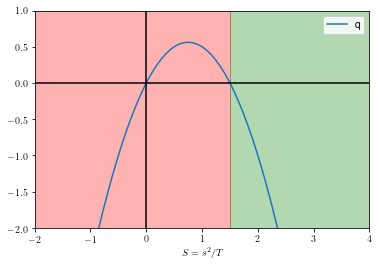
\includegraphics[width=.47\textwidth]{Images/qcas1.png} & 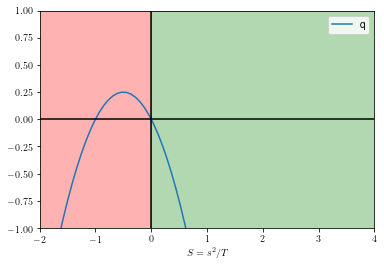
\includegraphics[width=.47\textwidth]{Images/qcas2.png} \\
\end{tabular}
\\
ii) Deux cas possibles sur la condition $q(S)^2-4\sigma(S)>0$:\\

\begin{tabular}{cc}
Une racine positive. & Trois racines positives. \\
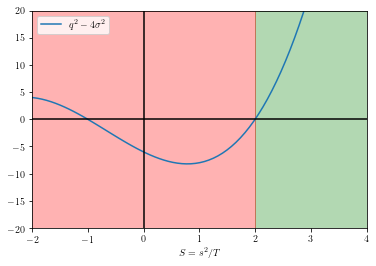
\includegraphics[width=.47\textwidth]{Images/q2cas1.png} & 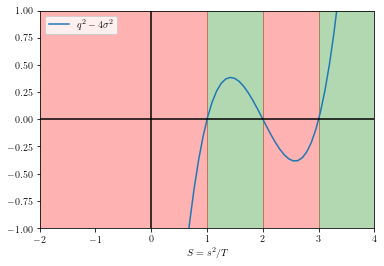
\includegraphics[width=.47\textwidth]{Images/q2cas2.png} \\
\end{tabular}
iii) Deux cas possibles sur la condition $\Delta_A(S) >0$:\\

\begin{tabular}{cc}
Trois racines négatives. & Une racine négative et deux positives.\\
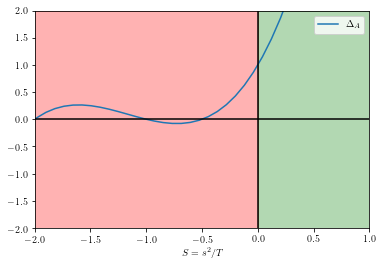
\includegraphics[width=.47\textwidth]{Images/deltacas1.png} & 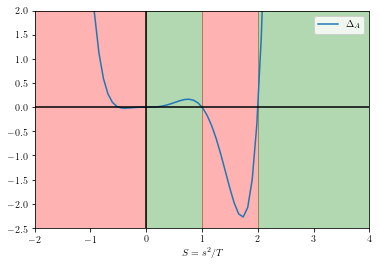
\includegraphics[width=.47\textwidth]{Images/deltacas2.png} \\
\end{tabular}







\subsection{Détermination de la vitesse d'onde extrémale $s$ par méthode d'extremum}
Soit $Y$ une racine de l'équation \ref{eq:PY}, $s$ est déterminé par $Y$ par l'équation: \begin{equation}
	s^2 = -\frac{Y^4}{P_3(Y)}. \label{eq:sfromY}
\end{equation} 
On cherche le plus grand $s<0$ (ou plus petit $s<0$) tel que les racines de \ref{eq:PY} soit toutes réelles (condition d'amortissement fort), donc nécessairement: \begin{equation}
	\frac{\partial s}{\partial Y}=0
\end{equation}
Ainsi: \begin{equation}
	\Big(\frac{Y^4}{P_3(Y)}\Big)'=0
\end{equation} 
i.e. \begin{equation}
\label{eq:Q}	Q(Y)\equiv4P_3(Y)-YP'_3(Y)=0
\end{equation}
Le polynôme $Q$ ne dépend pas de $s$, on peut donc calculer ses racines réelles (il en a une ou trois). Un calcul formel montre que son discriminant $\Delta _Q$ est positif: \begin{multline*}
\Delta _Q = 128F_0^5f_0^5 + 36 F_0^4 \lambda^2 f_0^4 + 192 F_0^4 \lambda f_0^5 + 192 F_0^4 f_0^6 + 108 F_0^3 \lambda^4 f_0^3 + 252 F_0^3 \lambda^3 f_0^4 + 240 F_0^3 \lambda^2 f_0^5 \\+ 192 F_0^3 \lambda f_0^6 + 96 F_0^3 f_0^7 + 36 F_0^2 \lambda^4 f_0^4 + 88 F_0^2 \lambda^3 f_0^5 + 84 F_0^2 \lambda^2 f_0^6 + 48 F_0^2 \lambda f_0^7 + 16 F_0^2 f_0^8 > 0
\end{multline*} donc $Q$ a trois racines.\\
On obtient donc au plus trois candidats négatifs pour $s$ par la formule: \begin{equation*}
	s^2 = -\frac{Y^4}{P_3(Y)}.
\end{equation*}
Le $s$ recherché est alors parmi ces candidats et peut être déterminé par le test suivant: \\

\begin{algorithm}[H]
\SetAlgoLined
\KwResult{Vitesse d'onde extrémale $s$ de l’équation d'onde associée au fluide}
 Entrées: données $\lambda$, $f_0$, $F_0$, $T$ et un $\epsilon$ choisi petit\;
 Calculer les racines réelles $y_i$ du polynôme $Q$ défini par \ref{eq:Q}\; 
 Candidats = $[]$\;
 \For{$y_i$ racine réelle de $Q$}{\If{$P_3(y_i)<0$}{Poser $s_i^2 = -\frac{y_i^4}{P_3(Y_i)}$ avec $s_i<0$\;
 Candidats $+=$ [$s_i$]}
 {}}
 \For{$s_i \in$ Candidats}{\If{le polynôme $Y^4 +(s_i^2-\epsilon)P_3(Y)$ n'a pas 4 racines réelles}{Candidats = Candidats \textbackslash $\{s_i\}$}}
 $s= \max$(Candidats)
 \caption{Recherche de la vitesse d'onde pour l’équation fluide}
\end{algorithm}
 \ifdefined\COMPLETE
\else
\end{document}
\fi